\section{A suitable CORBA test architecture\label{CORBA}}

CORBA is a standard promoted by the OMG consortium (\emph{Object
Management Group}) which is widely accepted in the telecommunication
industry, and the main actors of this sector have made large
investments in this technology.

The CORBA standard defines a general model for distributed programming
addressing heterogeneity at different levels (hardware, operating
systems, networks and protocols, programming languages). CORBA can be
viewed as a software infrastructure allowing the interconnection of
heterogeneous pieces of software. CORBA is based on an object-oriented
approach and on the client/server model.  

The core level of a CORBA implementation is called an ORB
(\emph{Object Request Broker}). CORBA objects are described in a pivot
language called IDL CORBA. This language allows communication between
different programming languages (for instance C, C++, \textsc{COBOL}, Java,
ST80, ...). An IDL CORBA definition describes the interface of a
software and not a complete implementation. The IDL definitions are
stored in an interface repository. This repository is mainly used to
dynamically construct a method invocation (dynamic invocation
interface).

The choice of CORBA as a test environment is motivated by the
following reasons: (1)~The telecommunication companies are moving to
CORBA; (2)~CORBA is a distributed environment garantying the
transparency of resource location and communication, despite
heterogeneity; (3)~CORBA is well fit for a modular architecture like
the SIB approach of the IN (see
section~\ref{descriptif_specification}). 

%At the moment CORBA proposes mainly a synchronous mode of invocation
%even if asynchronous invocations can be processed by the dynamic
%invocation interface. 

%A test sequence is composed by:
%\begin{itemize}
%\item messages addressed to the components under test. A message is
%composed of four parts. 
%The first part allows to initialize the component. The second one
%represents the input signal.
%The third one allows to access the result produced by the input signal and
%the fourth sets the component to a given state;
%\item messages to observe. Each message is composed by a name, a target object
%and some arguments values. One should be aware that the observation
%order of messages is important.
%\end{itemize}

\subsection{Test architecture}

Following classical architectures proposed for telecommunication
protocols, such as those described in the ISO~9646 normalization, we
propose a CORBA test architecture based on two types of components
(testers and components under test)~\cite{luis}. These components can
be distributed on different workstations but we have just one tester.

The Hit-or-jump algorithm generates test sequences that are composed
by active and passive segments. For the tester this implies the
ability to stimulate the components under test and to compare the
output to the attended result (the active part) but also the ability
to observe the messages exchanged between the components under test
(the passive part). Each message is composed by a name, a target object
and some arguments values.

The tester has two parts (see figure~\ref{test_archi}). The first one
processes CORBA messages corresponding to the active part of the test
and the second one is an observer for the passive part of the test.
From a CORBA point of view, the first part is a generic CORBA client
object able to invoke any operation on any CORBA object. 
The CORBA naming service is used to resolve names used in the test sequences
on CORBA object references (called IOR). The implementation of this first
part uses intensively the dynamic invocation interface which allows to
dynamically construct invocations using the interface repository.
Testers must have a timer to detect livelocks and locks. 

The second part of our tester is more difficult to address because we have
to observe the invocations exchanged between the tested objects
without modifying their source code. Moreover, the programming
interface of ORBs do not offer any mechanism to observe the
invocations. We have studied different solutions to this problem:

\begin{itemize}
  \item \emph{Extend an ORB with such capability.} This solution is more
        powerful because we can add any functionality we want but is
        also more difficult to realize. \cite{geib99} is an example of
        this approach. 

  \item \emph{Use interceptors.} Interceptors are a new functionality
        in the CORBA~2.3 standard. Interceptors allow to add some code
        during an invocation between a client and a
        server. Interceptors seem to be a good solution for our
        problem, unfortunately modification of the source code is
        necessary;

  \item \emph{Observe the invocations at the transport protocol
        layer.} CORBA~2 has standardized a communication protocol
        called GIOP (\emph{Generic Inter Orb Protocol}) to allow
        different ORBs to cooperate in order to transport an
        invocation message. GIOP allows interoperability between
        different ORBs. GIOP can have different incarnations depending
        on the transport layer used. IIOP (Internet Inter Orb
        Protocol) is the main incarnation of GIOP. IIOP uses TCP as a
        transport layer. This solution has several advantages for
        us. First it is independent of the ORB and second it does not
        imply any modification of the source code. The main drawback
        is that IIOP is a transport layer that ignores the semantic of
        the transported data. Another drawback is that IIOP is used
        for remote invocations but not for local invocations (many
        ORBs do some optimizations in the case of local invocations).
\end{itemize}

We have chosen the third solution but we have to force the distribution of
the components under test to ensure that all the invocations will be remote
ones. The software architecture of our tester is described
in figure~\ref{test_archi}.

\begin{figure}[htbp]
%\begin{center}
\centering
\centerline{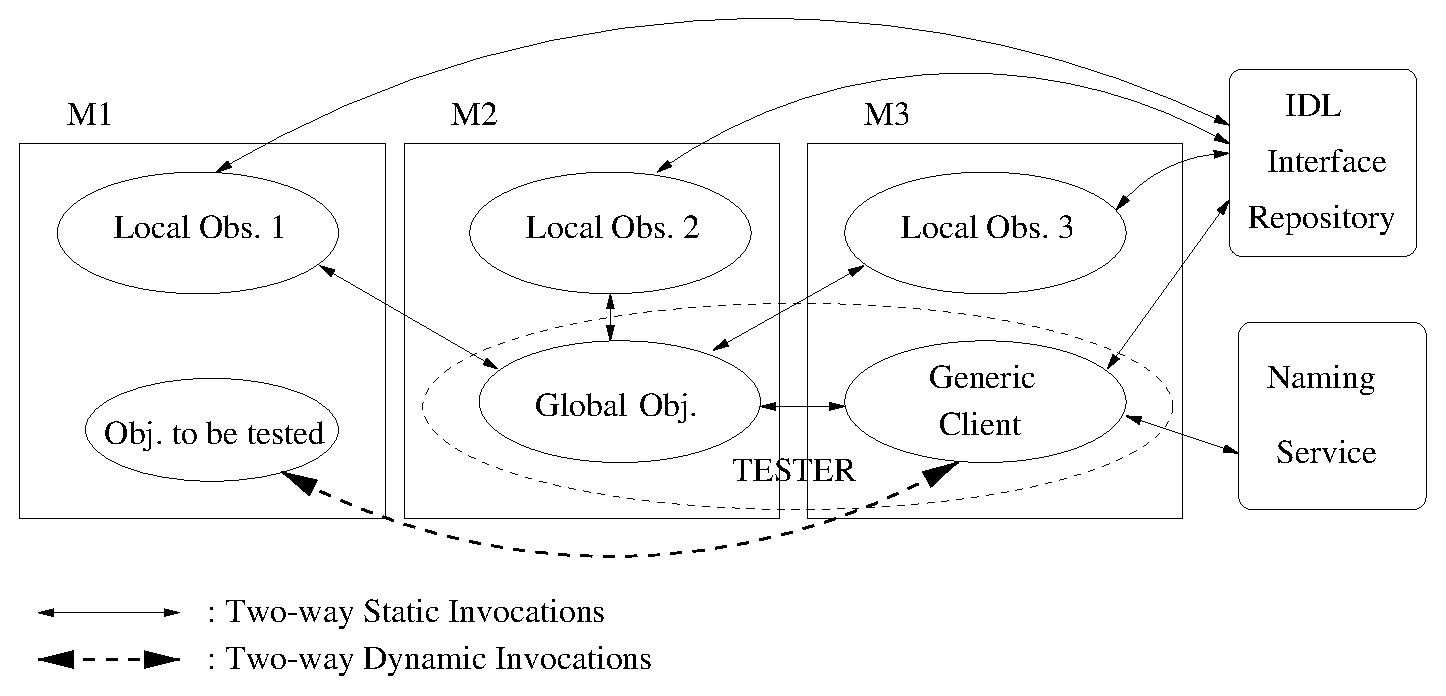
\includegraphics[width=8cm]{new_test_arch.eps}}
%\epsfxsize=11cm
%\epsfbox{test_arch.eps}
\caption{Tester architecture}
\protect\label{test_archi}
%\end{center}
\end{figure}

With the distribution constraint, we have to define a two-level
architecture for our observer. At the first stage we have one local
observer per workstation and at the second stage a global observer
which can be located at any site. Local observers and the global
observer has to cooperate in order to construct the global history of
invocations (this collaboration process is simplified because all the
invocations are synchronous). We have chosen CORBA as the distributed
infrastructure among the observers. The global observer interacts with
the tester using a CORBA IDL interface (so they may be located on
different sites). Interactions between the global observer and local
observers also use a CORBA IDL interface (in both directions). 


A local observer observes the local IIOP traffic and extracts useful
information from the segments
(name of the invoked operation, name of the target CORBA object
and value of the arguments, if any). The problem here is that IIOP
is a transport protocol and that we have to interpret the content of
the segment in order to extract the information we need. This
interpretation process uses the CORBA naming service to extract the
information about the target object and the interface repository to
extract the information about the invoked operation.\\
%Using the code generator of the ObjectGeode CASE from Verilog we have
%produced, from the SDL specification of the audio-conference service,
%an implementation in C language. We have focused on one component of
%this service which is the conference bridge process (it allows the
%reservation of a conference point terminal). In order to test
%completely this component using our testing platform, we have tried to
%encapsulate the generated code for this process in a CORBA server. To
%do this we have used a prototype developed by SEMA Group in an
%European project called SCREEN but without success. The CORBA
%encapsulation has to be done manually nd at this time we can not yet
%obtain the results of the execution of he test sequences generated by
%our platform.





